\section{Theory and Technical Backup}
\subsection{Hardware Features}
The robot's physical design is primarily anthropomorphic, incorporating elements inspired by animals as well. It stands approximately 12 inches tall and features various integrated hardware components. Starting from the top, the robot’s head will be a 3D-printed sphere with LED display eyes, which will serve as the primary form of interaction with the user. Additionally, the head will house a camera and microphone to capture images and sounds for processing by the microcontroller.
The robot’s body will consist of a large chassis designed to hold the servo motors and the PWM servo motor, which powers the movement of the arms, head, and base. A key feature of the design is the use of bevel gears arranged perpendicularly, enabling a compact structure while ensuring efficient power transmission. The robot will have a total of 4 degrees of freedom, incorporating mainly revolute joints driven by servo motors, which equally transmit power to the bevel gears, driving the base, arms, and head.
This design is similar to many desktop companion robots aimed at promoting mental wellness, such as Kiki or Eilik, with the primary distinction being the integration of various emotion detection methods. Throughout the first semester, the team iterated through many designs, and the final design was established as a bear-like robot shown in Figure \ref{fig:mockup}. 

\begin{figure}[ht]
    \centering
    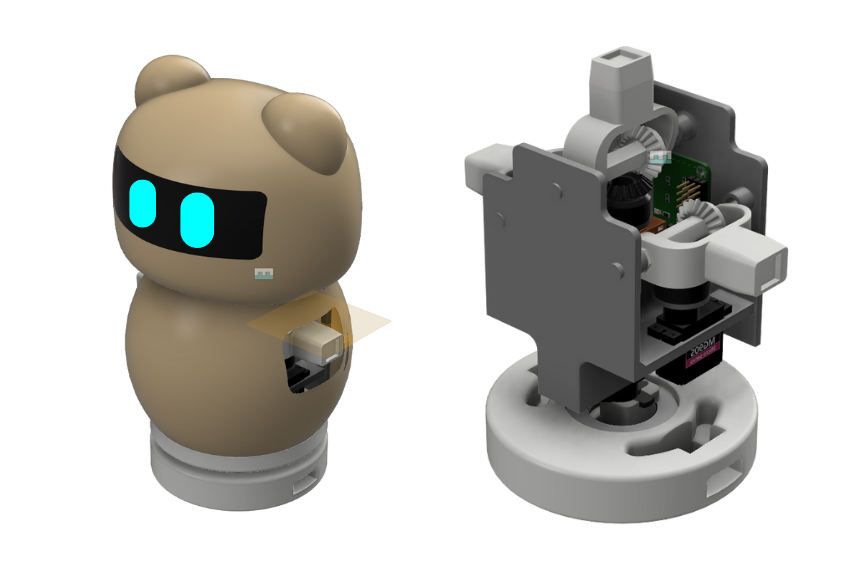
\includegraphics[width=\textwidth]{mockup.png}
    \caption{Pookie’s Mockup}
    \label{fig:mockup}
\end{figure}

In terms of high level system design, the system receives input from two sources: audio input and video input. The Jetson Nano processes these inputs and provides output through the speaker. The LCD output displays Pookie’s eyes. Additionally, the Jetson Nano controls the motor driver, enabling the movement of Pookie’s arm, base, and head mechanisms. The system also communicates with remote devices. Figure \ref{fig:arch} illustrates a high level diagram of all the components.

\begin{figure}[ht]
    \centering
    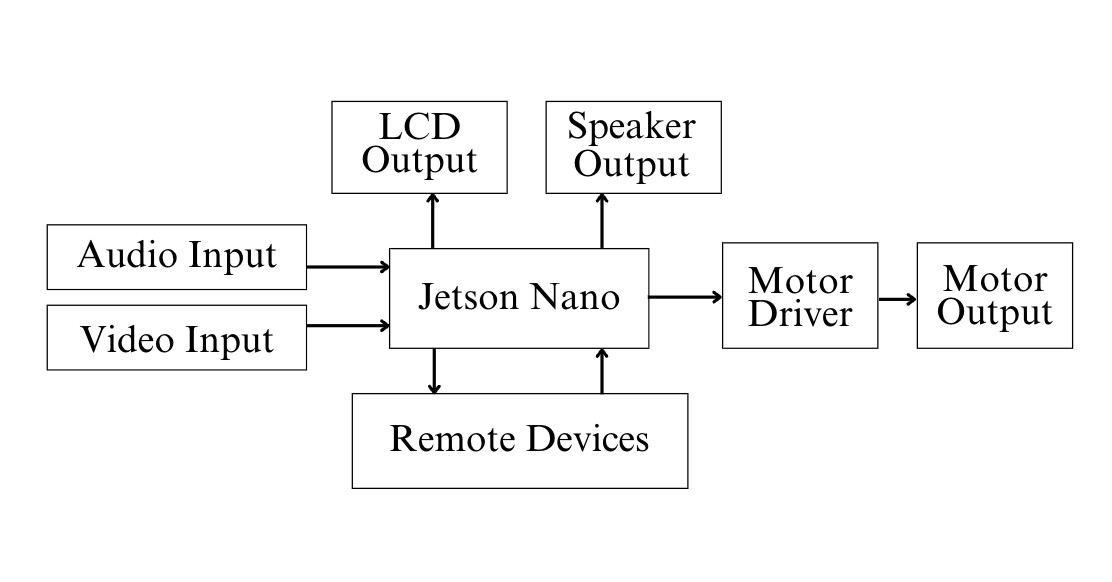
\includegraphics[width=\textwidth]{arch.png}
    \caption{High Level Architecture of the System}
    \label{fig:arch}
\end{figure}

\newpage
\subsection{Software Features - Overview}
The robot comprises two main features: emotion detection and interaction. Emotion detection is an initiative to incorporate empathy for the customer experience with the robot, using computer vision to analyze facial expressions, as well as speech emotion recognition to analyze tone and pitch. Given predicted emotional status, the robot will be programmed to provide interaction in two forms: verbal and non-verbal. Verbal interactions consist of noises made by the robot, whereas non-verbal interactions comprise physical actions from the robot such as arm movement or changes in the LED display resembling its eyes. Figure \ref{fig:soft_arch} illustrates the software architecture of the robot.

\begin{figure}[ht]
    \centering
    \captionsetup{justification=centering}
    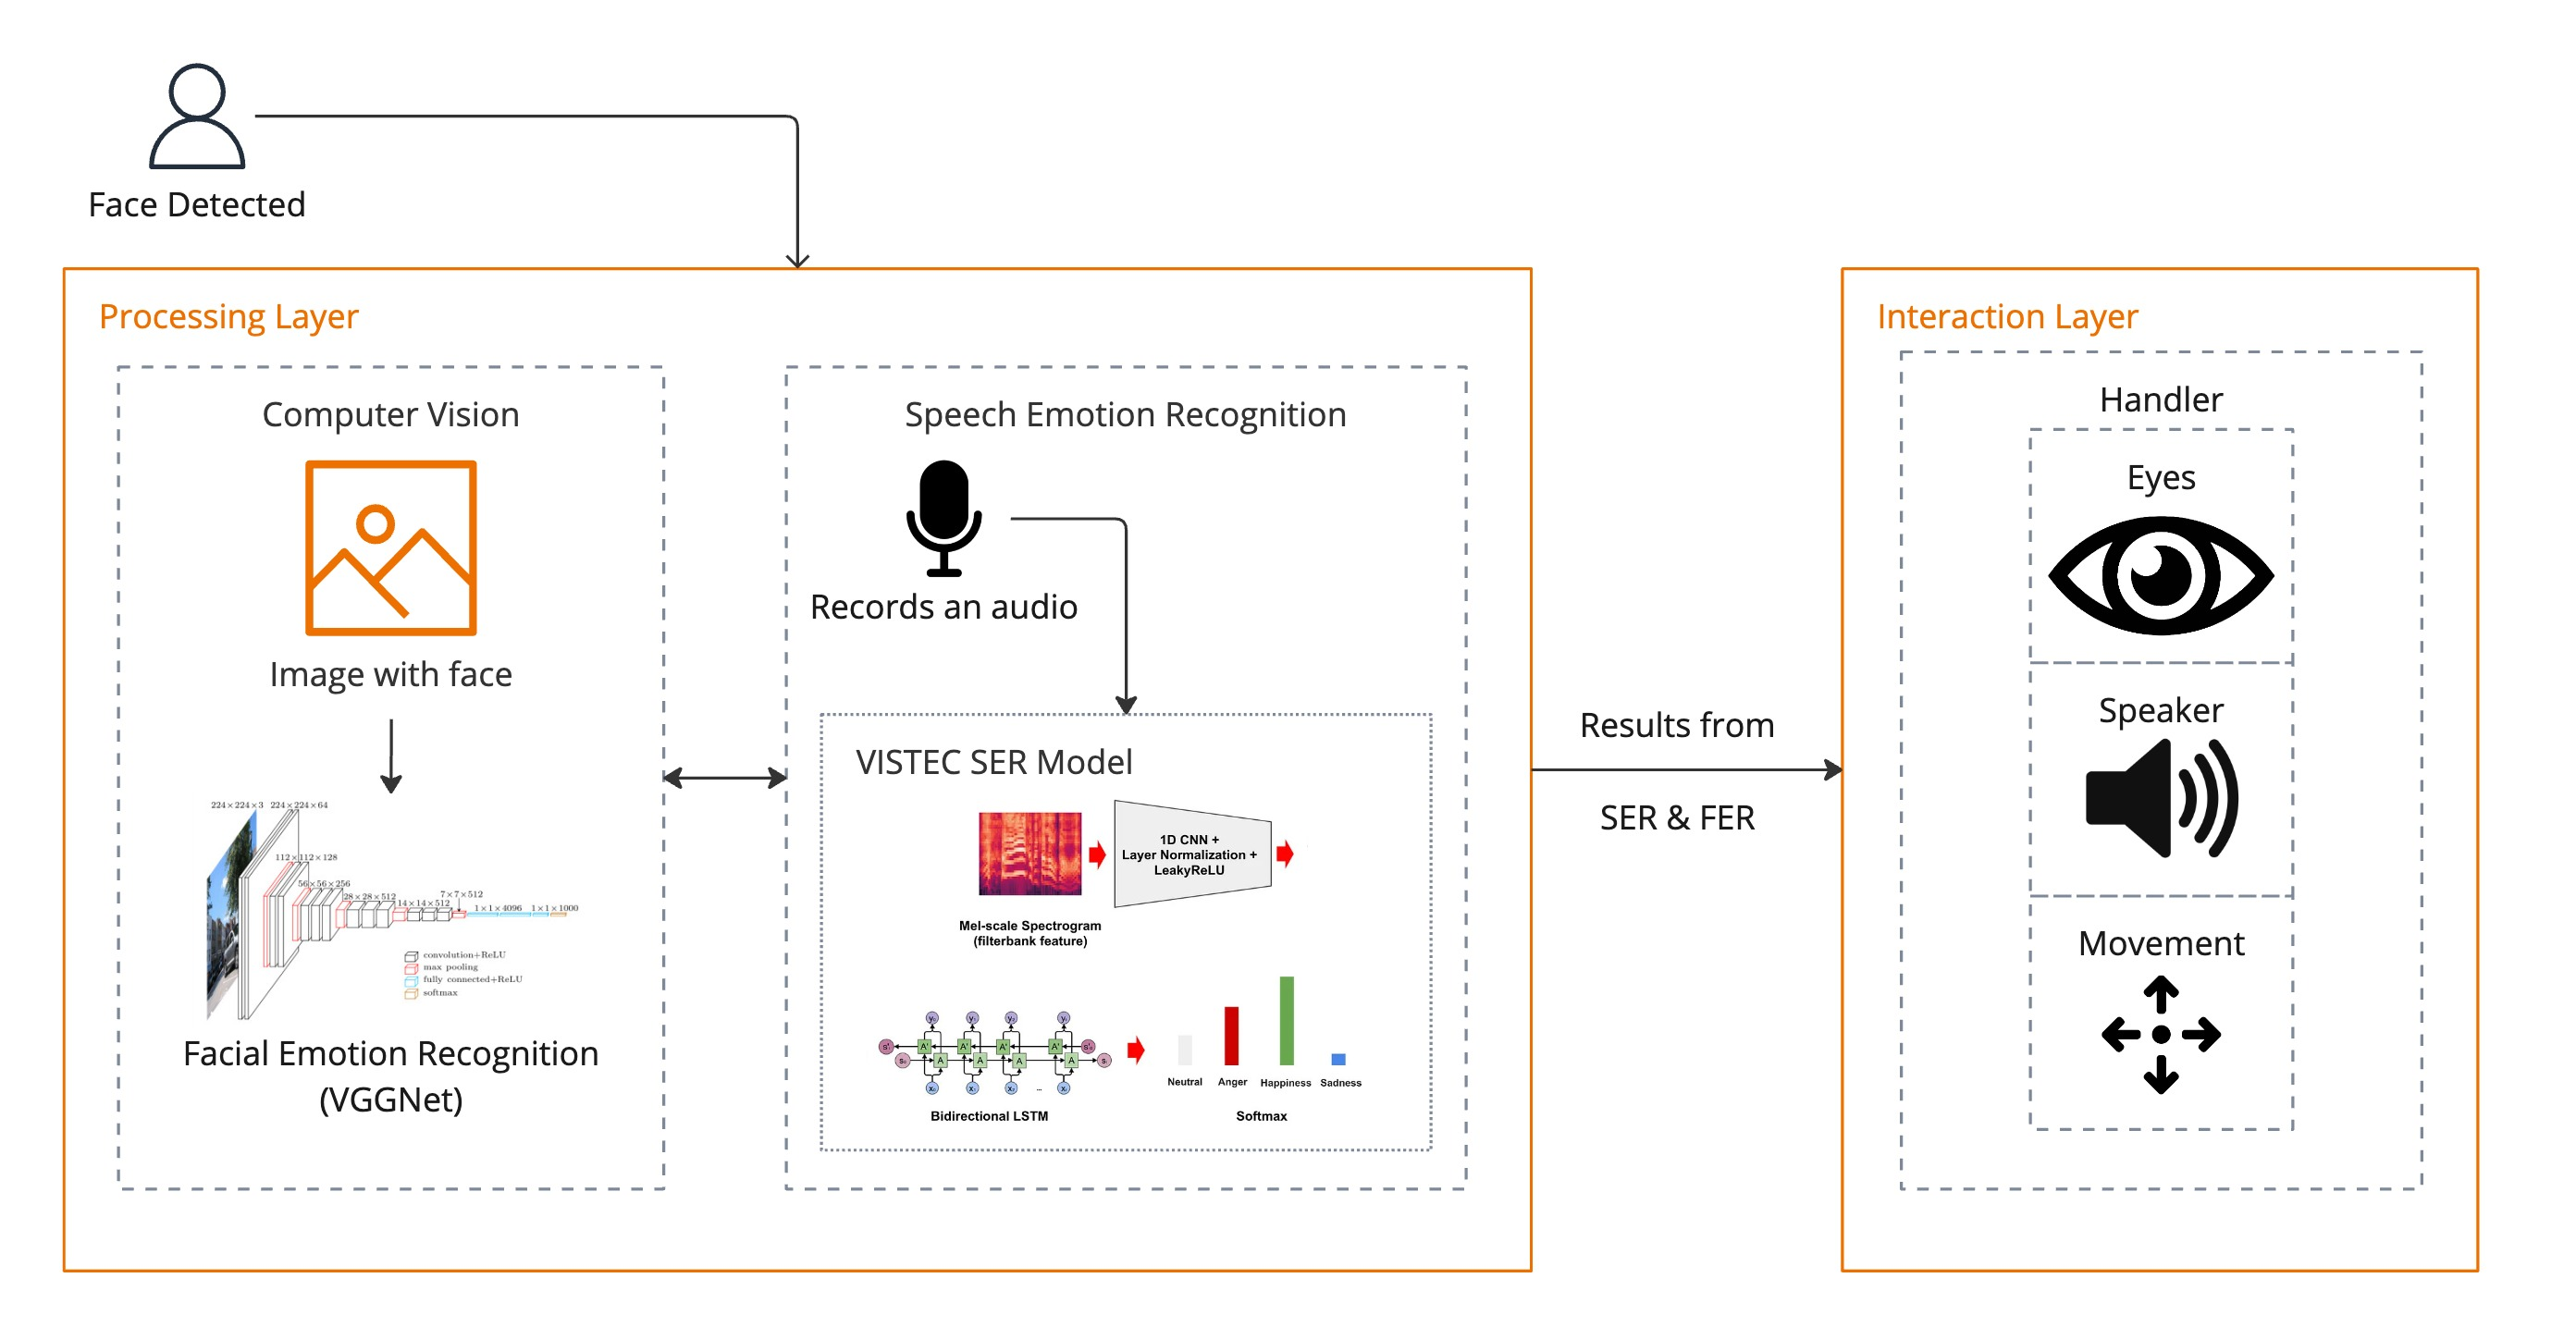
\includegraphics[width=\textwidth]{Flowchart.jpg}
    \caption{Pookie Software Architecture}
    \label{fig:soft_arch}
\end{figure}

\newpage
\subsection{Facial Expression Recognition}
Facial expression recognition is a core technique in emotion detection systems, crucial for understanding non-verbal emotional cues in humans. Recent advancements have centered on using Convolutional Neural Networks (CNNs) to detect and classify facial emotions with high accuracy. CNNs are particularly effective because they learn spatial hierarchies of features, enabling them to detect subtle changes in facial expressions, even in complex or dynamic environments. This capability makes CNNs highly suitable for emotion detection tasks, especially in applications requiring real-time emotion tracking, such as emotionally responsive robots.

One example in emotion classification is the integration of CNN-LSTM architectures \cite{RYUMINA2022435}, which improves how these models handle both the details in individual images and changes over time in a sequence of images. This is especially relevant in our project, as the testing dataset comprises Thai ethnicity, requiring robust generalization across unique facial features.

In this project, the emotion classification model maps facial expressions into 7 universal emotions, which must be further classified as stressed or anxious to fit the scope of the project. Research has shown that fear, anger, and disgust \cite{baltrusaitis2018} strongly correlate with stress and anxiety. Leveraging this finding, the robot detects these three emotions and, if present, performs specific action bubbles aimed at uplifting the user’s mood.

\subsection{Thai Speech Emotion Recognition}
Speech Emotion Recognition (SER) is an integral component of Pookie’s AI system, enabling it to interpret vocal emotional cues in Thai. By analyzing pitch, tone, and intensity, the SER system classifies emotions into five categories: neutral, anger, happiness, sadness, and frustration. SER is particularly effective because these vocal features are proven markers of emotional states, allowing accurate classification across a variety of speech patterns.

The model leverages a Thai-language dataset developed by Chulalongkorn University in collaboration with VISTEC, DEPA, and AIS, which contains 41 hours and 36 minutes of labeled audio recordings. Using this dataset, the SER model was developed by VISTEC and demonstrates a weighted accuracy of 66.12\% and an unweighted accuracy of 65.67\%.

The SER model performs best in recognizing neutral (0.72), anger (0.73), and frustration (0.61), while sadness (0.6) and happiness (0.62) exhibit slightly lower accuracies. However, notable misclassifications include frustration being confused with sadness (0.31) and happiness being confused with frustration (0.17). These misclassifications indicate areas for potential improvement, especially in distinguishing between similar emotions.

\begin{figure} [!htb]
    \centering
    \captionsetup{justification=centering}
    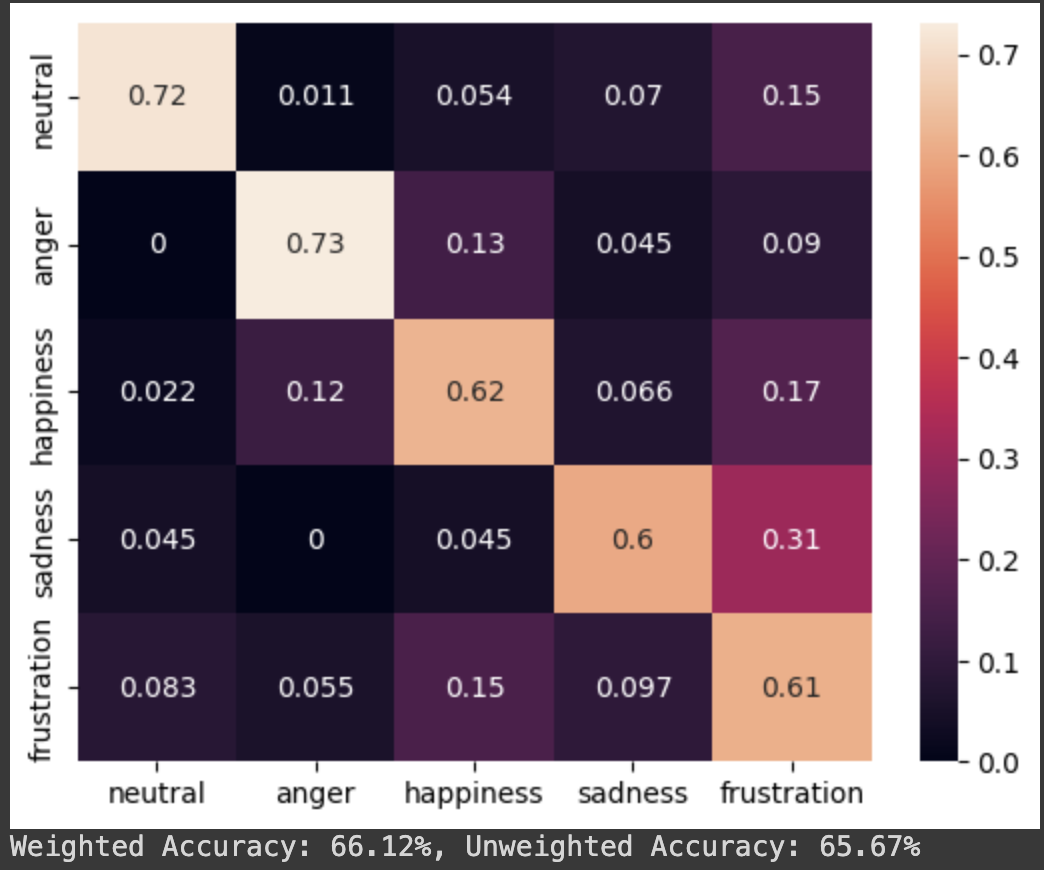
\includegraphics[width=0.5\textwidth]{ser_res.png}
    \caption{SER Confusion Matrix}
    \label{fig:ser-con}
\end{figure}

\subsection{Testing}

This section outlines the revised methodology for end-user testing, focusing on assessing the robot's ability to understand human emotions and deliver responses that positively impact the user’s mental state, particularly in reducing anxiety and promoting positivity. Since internal testing (e.g., model accuracy, integration testing) was thoroughly conducted last semester, this semester will emphasize external testing with real users.

Initially, the plan for end-user testing involved two participants, each interacting with the robot, Pookie, over the course of seven days. This approach was recommended by our psychology advisor, who believed that seven days would allow users to form an emotional attachment to the robot, which is essential for improving positivity in daily life. However, after consulting with our engineering advisor, Dr. Paulo, we were advised that testing with only two users would not provide statistically significant results. Consequently, the team decided to prioritize gathering more data points and deprioritize the focus on user attachment.

The final testing methodology will take place in a controlled environment: Pookie will be placed in the MI Innovation Labs, located in the 100th Year Engineering Building, for a period of 1–2 weeks. During this time, students will have the opportunity to interact with the robot and provide feedback. The MI Labs were chosen because they attract a high concentration of our target demographic (users aged 18 and above) and offer a safe, enclosed environment for testing. A team member will supervise the robot at all times, administering pre- and post-interaction surveys to gather data on changes in the users’ anxiety and positivity levels.

Although this approach provides a larger number of data points and allows for more robust data analysis, it does not fully replicate the intended user experience of incorporating Pookie into daily life, as originally envisioned. Given the time constraints, the team has opted for a method that prioritizes data collection over long-term user attachment.

One limitation of this method is the location itself: the MI Innovation Labs are frequented mainly by engineering students, which may skew the results. However, as our target demographic is users aged 18 and above with mild to moderate anxiety, engineering students can still serve as a reasonably representative sample for this segment.

The interactions will be brief, lasting approximately five minutes per user, excluding the time needed to explain the project. The specific parameters of the experiment are outlined in Table \ref{table:parameters}.

\begin{table}[h]
\centering
\caption{Experiment Parameters}
\label{table:parameters}
\begin{tabular}{|l|l|}
\hline
\textbf{Parameter} & \textbf{Details} \\ \hline
Format & Quantitative Questionnaire; Total 10 Questions \\ \hline
Environment & MI Innovation Labs, 100th Year Building, M Floor \\ \hline
Experiment Time & Approximately 5 minutes per person \\ \hline
HTarget Segment & Students aged 18 or more \\ \hline
\end{tabular}
\end{table}

As previously mentioned, users will be asked a series of questions before and after interacting with the robot, including some preliminary ones. For example, questions like "What is your occupation?" will help determine whether the robot has a more significant impact on specific user segments. Additionally, the numerical scores assigned will have specific interpretations, which we will later discuss with the psychology advisor (e.g., an anxiety score of 8 might indicate that the individual begins to struggle with tasks when anxious).

\subsubsection*{Preliminary Questions}
\begin{itemize}
    \item \textbf{Consensual:} Could you spare 5 minutes of your time for our experiment? We will collect data from you in the form of questionnaires, and we will only use your face and voice data temporarily for processing, where it will be completely erased afterwards, do you consent?
    \item \textbf{Demographic:} What is your age? What is your occupation? If you are a student, from which faculty are you studying?
\end{itemize}
\subsubsection*{Questions asked before interaction}
\begin{itemize}
    \item \textbf{Psychographic:} On a scale from 1-10, how would you rate your everyday positivity? 
    \item \textbf{Psychographic:} On a scale from 1-10, how frequently do you feel positive/happy? 
    \item \textbf{Psychographic:} On a scale from 1-10, how would you rate your daily anxiety levels?
    \item \textbf{Psychographic:} On a scale from 1-10, how frequently do you feel anxious?
\end{itemize}
